\documentclass[conference]{IEEEtran}
\usepackage{amsmath,amssymb,amsfonts}
\usepackage{algorithmic}
\usepackage{graphicx}
\usepackage{textcomp}
\usepackage{xcolor}
\usepackage{biblatex}
\usepackage{titlesec}
\usepackage{float}
\usepackage{listings,xcolor}



\def\BibTeX{{\rm B\kern-.05em{\sc i\kern-.025em b}\kern-.08em
		T\kern-.1667em\lower.7ex\hbox{E}\kern-.125emX}}


\addbibresource{references.bib}

\begin{document}

	
\title{Speaker Voice Similarity Analysis and Evaluation}

	
\author{\IEEEauthorblockN{Carmel Gafa}
	\date{April 2025}
	
}

\maketitle

\begin{abstract}
This study investigates the effectiveness of a WavLM-based system in distinguishing between 285 different speakers from the ABI-1 dataset. \end{abstract}



\section{Introduction}

Speaker identification is the determination of a speaker's identity from a segment of their speech. It is crucial in applications such as personalized voice assistants, security systems, and partitioning audio streams according to each speaker's identity. Unlike speech recognition, which focuses on what is being said, speaker identification is concerned with who is speaking.

This task can effectively be approached as a downstream application of pre-trained self-supervised speech models, such as \texttt{Wav2Vec2}\cite{baevski2020wav2vec} or its enhanced variant \texttt{WavLM}\cite{chen2022wavlm}. These models are trained on large-scale unlabelled audio datasets to learn audio representations that capture phonetic and speaker-specific characteristics.

In this project, \texttt{WavLM-base-plus-sv}, a fine-tuned version of \texttt{WavLM} specialized for speaker verification, is used to extract speaker embeddings from audio samples. These embeddings are compared using cosine similarity to measure the similarity of two voice samples. This architecture enables a simple speaker identification pipeline without the need to train a model from scratch.


\section{Data preprocessing}
\label{sec:data-processing}

The Accents of the British Isles (ABI) Corpus represents 13 regional accents. Figure \ref{fig:img-abi-corpus-accents} shows how these accents are categorized into four broad accent groups; Scottish, Irish, Northern English, and Southern English. Each broad group is further split into its respective regional accents\cite{najafian2016improving}.

\begin{figure}[H]
	\centering
	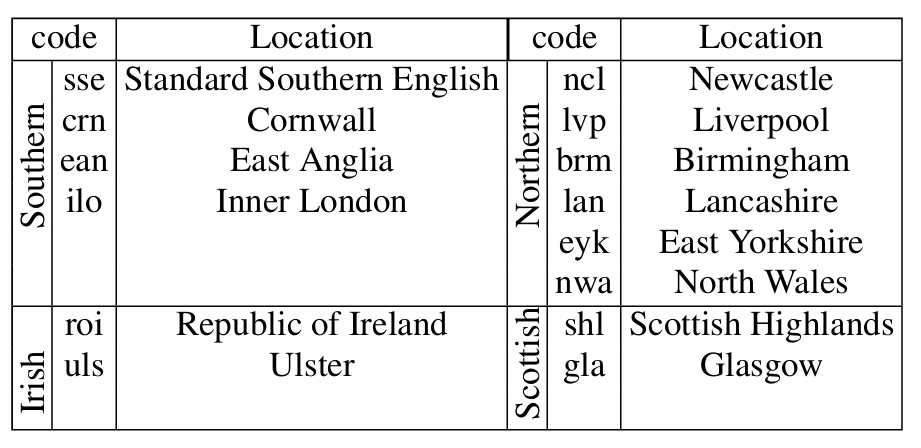
\includegraphics[width=0.7\linewidth]{img/img-abi-corpus-accents}
	\caption{Accents represented by the ABI Corpus\cite{najafian2016improving}.}
	\label{fig:img-abi-corpus-accents}
\end{figure}

The corpus includes 285 subjects, with speech collected from individuals who have lived in each regional accent area since birth. Each of the 285 subjects read the same three short passages. These are short paragraphs forming the 'sailor passage', with lengths of 92, 92, and 107 words with average durations of 43.2, 48.1, and 53.4 seconds, respectively\cite{najafian2016improving}.

The sources do not explicitly describe the recording conditions of the ABI corpus, however, it is mentioned that the speakers were selected by a phonetician, suggesting an effort for a standard quality recording for at least that accent\cite{najafian2016improving}.

\subsection{Signal resampling}
\label{ssec:signal-resampling}

Audio signals depend on two main parameters

\begin{itemize}
	\item number of channels $C$, that is $1$ for mono and $2$ for stereo.
	\item number of samples $T = t \times f_s$; that in turn depends on the
	\begin{itemize}
		\item duration $t$ of the audio in seconds.
		\item sampling rate $f_s$ (e.g. 48,000 Hz).
	\end{itemize}
	
\end{itemize}

For a mono signal, that is common in these applications, a vector representing the utterance is available for processing,  $\mathbf{x}_{\text{raw}} \in \mathbb{R}^{1 \times T}$ in this way.


The model by Microsoft that we are using in this example expects a signal rate of 16,000 Hz, and it is therefore necessary to resample the signal to this frequency. The resampling step involves selecting a subset of samples from the original vector, so that the original sampling rate $f_s^{\text{raw}}$ becomes a lower one $f_s^{\text{target}}$. The down-sampling ratio in this case, $R = \frac{f_s^{\text{raw}}}{f_s^{\text{target}}} = 3$


Before reducing the number of samples, the high-frequency components from the original signals are removed, as they could cause aliasing. Aliasing occurs when frequencies above the new Nyquist frequency (which is one-half the new sampling rate) “fold back” into the signal, corrupting it. The Nyquist frequency after down-sampling becomes:

$$f_N^{\text{new}} = \frac{f_s^{\text{target}}}{2} = 8000~\text{Hz}$$

To remove the high frequency components, a low-pass filter is applied, generating a filtered signal, $\tilde{x}$

$$\tilde{x}[n] = x_{raw}[n] * h[n]$$

where $h[n]$ is the impulse response of a low-pass filter, typically a windowed \texttt{sinc} function:

$$h[n] = \text{sinc}\left(\frac{n}{R}\right) \cdot w[n]$$

Here, $w[n]$ is a window function (like Kaiser, Hamming, etc.) to localize the infinite \texttt{sinc} filter in time.

If, as an example, we consider this function:

\begin{align*}
	x_{raw} &=[x[0], x[1], x[2], x[3], x[4], x[5], x[6], x[7], x[8]]\\
		 	&=[2, 4, 6, 8, 10, 8, 6, 4, 2]
\end{align*}

and use the following windowed \texttt{sinc} filter (kernel)

\begin{align*}
	h &= [h[0],\ h[1],\ h[2]]\\
	  &= [0.2,\ 0.6,\ 0.2]
\end{align*}

We slide the kernel over the signal and compute:

$$\tilde{x}[n] = \sum_{k=0}^{2} x[n + k] \cdot h[k]$$

So that the first two samples of the filtered signal becomes

\begin{align*}
	\tilde{x}[0]	&= 0.2 \cdot x[0] + 0.6 \cdot x[1] + 0.2 \cdot x[2] \\
					&= 0.2\cdot2 + 0.6\cdot4 + 0.2\cdot6 \\
					&= 0.4 + 2.4 + 1.2 \\
					&= 4.0\\
	\tilde{x}[1] 	&= 0.2 \cdot x[1] + 0.6 \cdot x[2] + 0.2 \cdot x[3] \\
					&= 0.2\cdot4 + 0.6\cdot6 + 0.2\cdot8 \\
					&= 0.8 + 3.6 + 1.6 \\
					&= 6.0
\end{align*}

Once the signal is filtered, we can keep every $R^\text{th}$ sample and discard the rest (decimation), or alternatively, apply interpolation to produce a smoother, resampled signal at the desired rate.

$$x_{\downarrow R}[n] = x[Rn]$$

So that, for example,

$$x_{\downarrow 3}[n] = x[0], x[3], x[6], x[9], \dots$$


\begin{figure}[H]
	\centering
	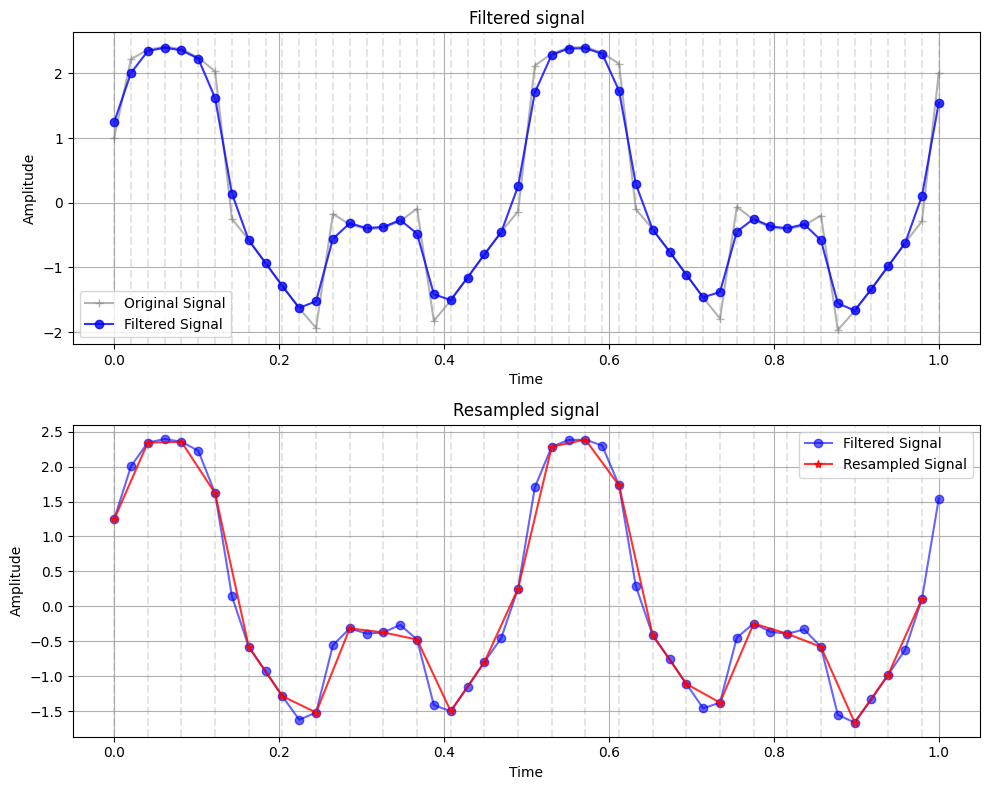
\includegraphics[width=0.9\linewidth]{img/img-resampling}
	\caption{}
	\label{fig:img-resampling}
\end{figure}




\section{Methodology}

In this section, we will discuss the implementation of the speaker voice similarity comparison pipeline. Several general criteria were observed during this exercise:
\begin{itemize}
	\item Code that manipulated data was implemented in Python scripts, whereas code that analysed data in Python notebooks. This approach is preferred for several reasons:
	\begin{itemize}
		\item Scripts encourage modularity better.
		\item It is easier to import developed functions when using scripts.
		\item Scripts avoid the notebook's overheads like kernel restarts and variable state issues.
		\item The notebooks' interactive nature makes them very attractive for data analysis and tasks with a predominant visualisation component.
	\end{itemize}
	\item The analysis of voice similarity is broken down into discrete steps and implemented as stand-alone modules.    Each module will generate one or more results that are, in most cases, based on the results generated by previous modules in the pipeline. This approach is inspired from the medallion architecture that is widely used in industry.
	\item Modules are stringed logically together to perform all the tasks necessary in this project, including the download of the data and model.
	\item Data is manipulated only using code. The whole project can be executed without any manual intervention whatsoever.
	\item Wherever possible, an option to execute the appropriate parts of a module on the GPU was made available.
	\item A simple logging tool was created so all modules can inject information about their execution. This logger is also used by a timer decorator that was created to measure the duration of the various modules of this project.
\end{itemize}

\subsection{Comparison strategy}
\label{ssec:comparison-strategy}

As discussed in Section \ref{sec:data-processing}, three audio files are available for each speaker in the ABI-1 dataset, and these will be used to determine the similarity of any speaker to all other speakers in the dataset. The following approach is used to determine similarity in this exercise.

Each audio file is compared with the other audio files for a given speaker, a total of four comparisons, and the minimum value is retained as the self-comparison result.

For every speaker combination in the dataset, each audio file of one speaker is compared to all the audio files of the other speaker, a total of nine comparisons and the maxim value is retained as the inter-comparison result.

This approach will determine the thresholds and results that provide, beyond any doubt, the best separation possible, as the minimum distance between self and inter-comparisons will be examined.



\subsection{Voice similarity comparison pipeline}

\begin{figure}[H]
	\centering
	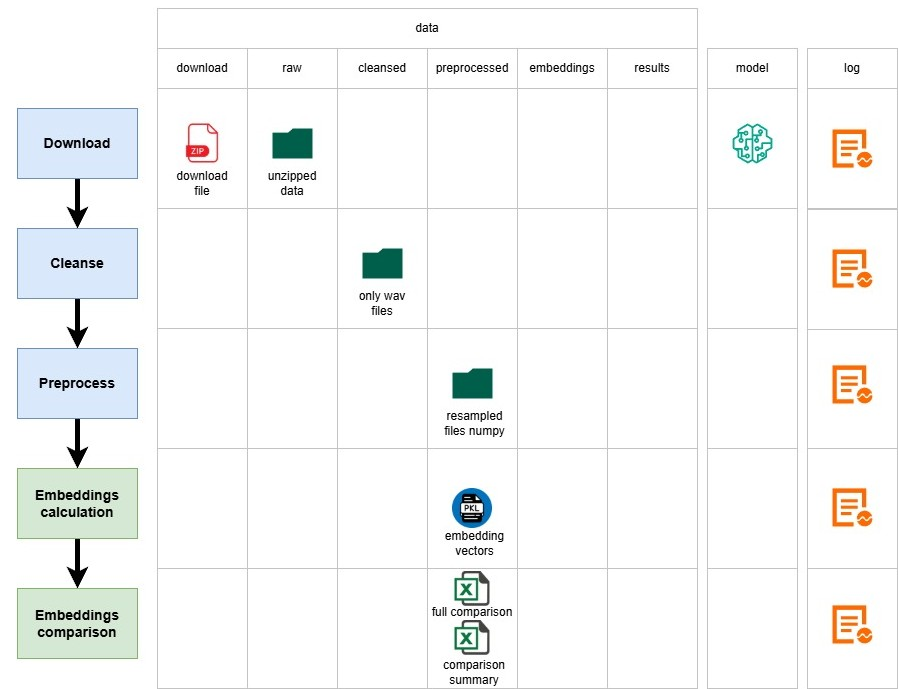
\includegraphics[width=1\linewidth]{img/img-pipeline}
	\caption{}
	\label{fig:img-pipeline}
\end{figure}

Figure \ref{fig:img-pipeline} shows the flow that was implemented as part of this project, which is made up of the following modules:
\begin{itemize}
	\item \textbf{Download}. In the first step of the pipeline, the \texttt{ABI-1} dataset archive is downloaded and placed in the \texttt{data/download} folder. The contents are then extracted and placed in the \texttt{data/raw folder}. The \texttt{ABI-1} structure has an \texttt{accents/genders/speakers} structure, whereby accents folders contain a male and female folder for each speaker. At this point, the data also contains additional data, such as transcription information.
	The \texttt{wavlm-base-plus-sv} model is also downloaded and placed in the \texttt{model} folder.
	This module also contains the functionality to create the data, module and log folder structure that is necessary for this project.
	
	\item \textbf{Cleanse}. In the next step, the contents of each speaker, in each gender and each accent in the raw data are examined, and the files having a "\texttt{.wav}" extension are retained. The results are placed in an identical folder structure in the \texttt{data/cleansed} folder.
	
	\item \textbf{Preprocess}. As we have discussed in Section \ref{ssec:signal-resampling}, the audio files need are preprocessed to 16KHz so that their embeddings can be evaluated by the model. In this next step, all the audio files of each speaker, in each gender and accent in the raw data folder are loaded and resampled. The resulting \texttt{numpy} arrays are placed in an identical folder structure in the \texttt{data/preprocessed} folder.
	
	\item \textbf{Embedding calculation}. In the next step, the \texttt{wavlm-base-plus-sv} model calculates the embeddings for each audio data file. Each embedding is effectively a 512-element vector, so a $3 \times 512$ array is created for each speaker. The embedding information was stored in a dictionary data structure with "\texttt{accent-gender-speaker}" as key and the embedding array as the value during processing. It was then converted to a\texttt{pandas} \texttt{DataFrame} and saved as a pickle file in the \texttt{data/embeddings}.
	
	\item \textbf{Comparison}. The final step of the pipeline implements cosine-similarity comparison using the strategy explained in Section \ref{ssec:comparison-strategy}. Two files are generated in this process:
	\begin{itemize}
		\item A raw results file contains the results of all comparisons: a set of three for self-comparison and a set of nine for inter-comparison.
		\item A summary results file that contains the selected comparison from each set using the comparison strategy.
	\end{itemize}
	The result files are stored in the \texttt{data/results} folder
\end{itemize}





\subsection*{Embedding Extraction Using the WavLM Model}
I used the pre-trained \texttt{microsoft/wavlm-base-plus-sv} model, downloaded locally from Hugging Face using the \texttt{transformers} library. The model was loaded in evaluation mode and used to generate speaker-level embeddings through \texttt{WavLMForXVector}. Input waveforms were prepared via the associated \texttt{Wav2Vec2FeatureExtractor}, ensuring correct sampling rate and tensor formatting.

\subsection*{Audio Preprocessing}
Only audio files matching the pattern \texttt{shortpassage*.wav} were retained from the ABI-1 Corpus. Each file was resampled to 16\,kHz using \texttt{torchaudio.transforms.Resample} and saved as NumPy arrays (\texttt{.npy}) for efficient processing. This ensured compatibility with the WavLM model while reducing preprocessing overhead during embedding extraction.

\subsection*{Aggregation and Similarity Computation}
Each speaker’s embeddings were aggregated by concatenating all available utterance-level vectors. Pairwise cosine similarities were computed for:
\begin{itemize}
	\item Intra-speaker comparisons (same speaker, different recordings)
	\item Inter-speaker comparisons (different speakers)
\end{itemize}
The \texttt{torch.nn.CosineSimilarity} function was used to calculate similarity values. These were saved into both raw and summary CSV files for further evaluation.

\subsection*{Dimensionality Reduction and Visualization}
To analyze speaker embedding separability, I plotted cosine similarity distributions using \texttt{seaborn} histograms and KDE curves. Separate visualizations were generated for:
\begin{itemize}
	\item Same-speaker pairs
	\item Different-speaker same-gender pairs
	\item Cross-gender speaker pairs
\end{itemize}
Range plots were used to highlight typical similarity intervals, offering visual guidance on threshold selection.

\subsection*{Threshold Selection and Accuracy Evaluation}
Several thresholds were tested to distinguish between "same" and "different" speaker pairs. Using these thresholds, identification accuracy was computed as the proportion of correctly labeled pairs over total comparisons. Descriptive statistics and distribution plots supported the choice of an optimal threshold that maximized true positives while minimizing false positives.

\subsection*{Confusion Matrix Analysis}
Confusion matrices were generated at varying thresholds to measure classification performance in terms of true positives, false positives, true negatives, and false negatives. These matrices helped identify critical error patterns and assess the system's robustness under different decision boundaries.

\subsection*{Experimental Setup and Execution Pipeline}
The full experiment was orchestrated using the script \texttt{execute\_pipeline.py}, which sequentially executes:
\begin{enumerate}
	\item Dataset and model download
	\item Data cleansing and preprocessing
	\item Embedding extraction
	\item Similarity computation and analysis
\end{enumerate}
Speaker IDs followed a standardized \texttt{Accent-Gender-SpeakerID} format and were later expanded for analysis of accent, gender, and individual trends.






\section{Evaluation and results}


\section{Analysis and discussion}

\section{Conclusion and future work}




\section*{Generative AI}

\printbibliography


	
\end{document}
